\documentclass[a4paper]{article}
\usepackage{graphicx}
\begin{document}
part1

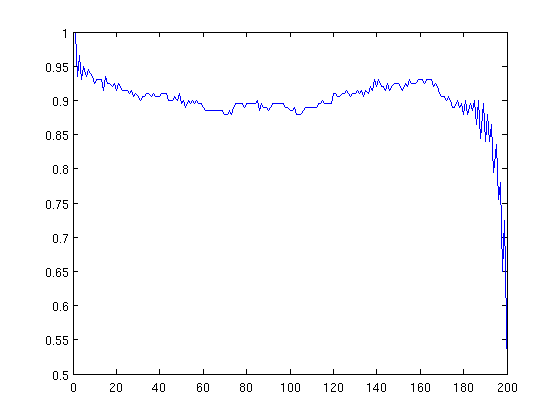
\includegraphics[scale=0.2]{1}
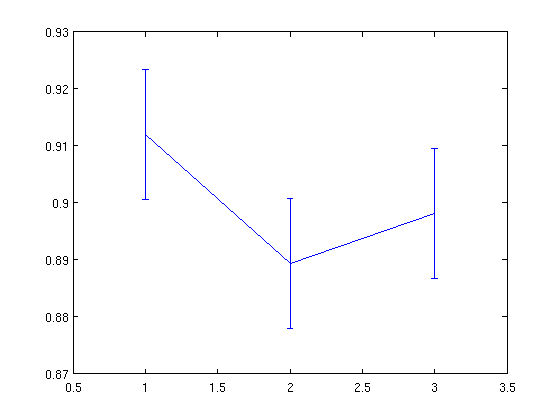
\includegraphics[scale=0.2]{2}

the k = 1 means that the data is classified by the nearest 1 data.
for example, in the diagram, a point is classified by the nearest point.
when k get bigger the accuracy will decrease as the diagram show.

the second diagram is a bit different with the first one, it is because the
data we used is too less, more data we used, the two diagrams get more similar.

the third diagram used three set of data to show the accuracy and error bar.

for parte, use three label to mark the 3 types of data 3 6 8, and try to
calculate the accuracy.

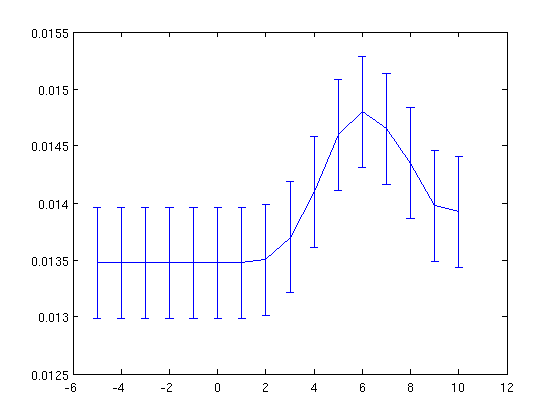
\includegraphics[scale=0.2]{3}
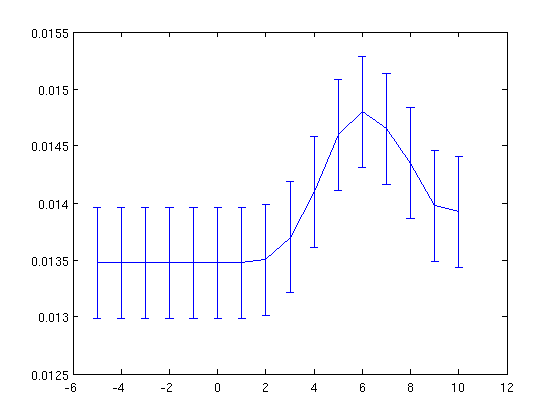
\includegraphics[scale=0.2]{4}
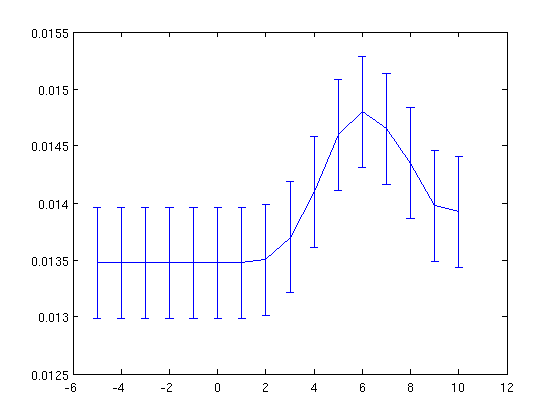
\includegraphics[scale=0.2]{5}
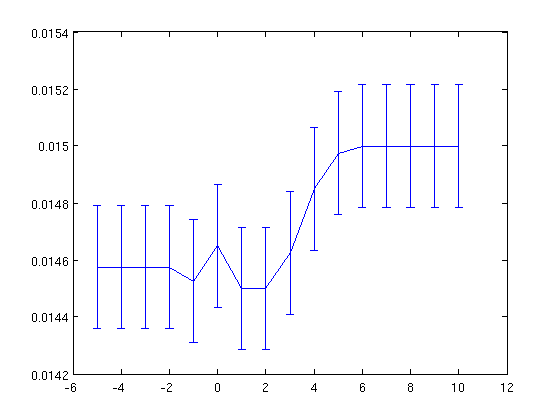
\includegraphics[scale=0.2]{6}

lambda is used to regularise the data, when it is = 0, it means there is no regularise.
so the accuracy will not be very high with no regularise.
for the part2, i use some diagram to perform the relationship with lambda and
accuracy. So i can choose a best lambda value to regularise the data.

the trainning takes a second use the method in b.
for partd, i get the similar diagram as partc.
for parte, i use the best lambda value to regularise the data and get a very high accuracy.


part3 is similar to part2, but i change the label to 3 6 8 their self.
for accuracy, i compare the diagram to check the distance of the line to 3 6 8.
i used the same method in part2 to choose the best lambda.
but the accuracy is not very high, i think more sample data is needed rather than
just using 200 for each types of data if there is three types of data. 
\end{document}
